\documentclass[10pt,a4paper]{article}

\usepackage[utf8]{inputenc}
\usepackage[T1]{fontenc}
\usepackage[spanish,es-nodecimaldot]{babel}
\usepackage{lmodern}
\usepackage{microtype}
\usepackage[a4paper,margin=1.45cm,top=1.25cm,bottom=1.3cm]{geometry}
\usepackage{amsmath,amssymb}
\usepackage{booktabs,array,tabularx}
\usepackage{graphicx}
\usepackage{xcolor}
\usepackage{enumitem}
\usepackage{titlesec}
\usepackage{caption}
\usepackage[hidelinks]{hyperref}

\definecolor{azul}{HTML}{173B57}
\definecolor{dorado}{HTML}{B7791F}
\definecolor{gris}{HTML}{52606D}
\setlength{\parindent}{0pt}
\setlength{\parskip}{3.2pt}
\setlength{\tabcolsep}{4pt}
\renewcommand{\arraystretch}{1.08}
\titleformat{\section}{\large\bfseries\color{azul}}{}{0pt}{}
\titleformat{\subsection}{\normalsize\bfseries\color{azul}}{}{0pt}{}
\titlespacing*{\section}{0pt}{6pt}{2pt}
\titlespacing*{\subsection}{0pt}{4pt}{1pt}
\captionsetup{font=small,labelfont=bf,skip=3pt}
\pagestyle{plain}

\begin{document}

\begin{center}
    {\LARGE\bfseries\color{azul} Gold Dice RL}\par
    \vspace{2pt}
    {\large Trabajo Práctico 1 -- Reinforcement Learning}\par
    \vspace{5pt}
    \textbf{Agustín Chmielewski \quad Juan Pablo Saldungaray \quad Uriel Slavkin}\par
    \vspace{2pt}
    Inteligencia Artificial y Neurociencias -- UTDT
\end{center}

\section{Cómo encaramos el problema}

Al leer el enunciado nos quedaron tres preguntas: cuánto se puede obtener si se juega bien, qué parte de la observación necesita recordar el agente y cómo representar \texttt{SCORE}, que permite elegir cualquier cantidad de oro, dentro de una tabla con pocas acciones.

Uno de nosotros viene de competir en ICPC y reconoció un problema de horizonte finito. Antes de entrenar planteamos una programación dinámica (DP). Esta decisión cambió el trabajo: además de entrenar un agente, pudimos calcular una referencia y medir cuánto costaba cada simplificación.

\subsection{Por qué este juego admite una DP}

El ambiente cumple cuatro condiciones que permiten resolverlo hacia atrás:

\begin{enumerate}[leftmargin=17pt,itemsep=1pt,topsep=1pt]
    \item la partida dura 30 turnos;
    \item conocemos las probabilidades de dados y tormentas;
    \item conocemos el efecto y el costo de cada acción;
    \item el futuro depende de un estado pequeño.
\end{enumerate}

Definimos
\[
U_t(g,n,b,e)=\text{puntos esperados antes de tirar en el turno }t,
\]
donde $g$ es oro, $n$ dados, $b$ bonus y $e$ escudos. Los puntos acumulados no entran en el estado: suman al resultado, pero no modifican tiradas, precios ni tormentas. El valor guardado se incorpora al calcular la transición siguiente.

Después de la tirada observamos su suma $R$ y su máximo $M$. Para cada acción legal $a$ calculamos de forma determinista la recompensa inmediata $r_a$ y el estado posterior $F_a$. Luego integramos la tormenta y consultamos el turno siguiente:
\[
U_t(s)=\mathbb{E}_{R,M}\!\left[
\max_{a\in A(s,R,M)}\left(r_a+
\mathbb{E}_{\text{tormenta}}U_{t+1}(F_a)\right)\right].
\]

El caso base es el turno 30. No habrá otra tirada, por lo que conviene convertir todo el oro en puntos. Recorremos $t=30,29,\ldots,1$ y guardamos sólo dos capas. Calculamos la distribución conjunta $(R,M)$ por convolución, sin muestrear partidas. Para \texttt{SCORE(k)} usamos un máximo prefijo que evalúa todas las cantidades en $O(G)$, en lugar de $O(G^2)$.

El archivo \texttt{sol\_dp.cpp} implementa esta recurrencia en 92 líneas de C++17. Con los límites usados en el análisis imprime \textbf{642,452 puntos} desde el estado inicial. La DP no juega el torneo ni aprende de la experiencia; funciona como referencia calculada con conocimiento completo del ambiente.

\subsection{Una primera intuición que descartamos}

Pensábamos que reducir los cientos de valores posibles de \texttt{SCORE(k)} destruiría información. Resolvimos de nuevo la DP permitiendo sólo \texttt{SCORE(todo)} y obtuvimos el mismo valor dentro de la precisión usada. La política calculada cobra al final. El agente aprendido trabaja entonces con seis opciones: pasar, puntuar todo, comprar un dado, mejorar los dados, comprar un escudo o guardar el mejor dado.

\newpage
\section{El agente de Reinforcement Learning}

\subsection{Estado y recompensa}

La observación original tiene nueve campos. Nosotros aprendemos sobre el estado posterior a la acción, o \emph{afterstate}:
\[
(\text{turno},\text{oro},\text{dados},\text{bonus},\text{escudos},\text{guardado}).
\]
Una compra produce un efecto determinista; el azar aparece después, con la tormenta y la próxima tirada. Dos pares estado--acción que llegan al mismo \emph{afterstate} comparten experiencia. Sacamos los puntos acumulados porque no afectan el futuro; \texttt{roll\_sum} ya se sumó al oro y \texttt{roll\_max} sólo interviene al evaluar \texttt{STORE\_BEST\_DIE}.

El oro no tiene un límite declarado. Usamos una grilla no uniforme: conserva cada entero entre 0 y 96, donde se concentran los precios, y separa más los valores altos. Interpolamos entre nodos vecinos. Esta representación distingue 41 de 42 cuando 42 habilita una compra.

Conservamos la recompensa del ambiente: \texttt{SCORE} entrega como recompensa la cantidad convertida en puntos y las demás acciones entregan cero. Como gran parte de la recompensa llega al final, inicializamos el valor con
\[
\Phi=\text{oro}+\text{guardado}+5\,\text{escudos}
+\text{turnos restantes}\cdot\text{dados}\cdot(3{,}5+\text{bonus}).
\]
La tabla aprende una corrección sobre $\Phi$. Esta cuenta valora la caja y la producción esperada si no se comprara nada más. No contiene la probabilidad de tormenta ni decide cuándo conviene comprar; el agente aprende esas diferencias al jugar.

\subsection{Algoritmo e hiperparámetros}

El modelo entregado es \textbf{Q-Learning tabular sobre afterstates con Double Q-Learning}. Mantiene dos tablas. En cada actualización, una selecciona la mejor continuación y la otra calcula su valor. Elegimos esta variante porque una sola tabla empezó a empeorar al aumentar los episodios, un efecto compatible con el sesgo de maximización sobre estimaciones ruidosas.

\begin{center}
\small
\begin{tabular}{@{}lrp{8.2cm}@{}}
\toprule
Parámetro & Valor & Decisión \\
\midrule
Episodios & 1.500.000 & mejor checkpoint cada 100.000 \\
$\gamma$ & 1 & horizonte finito, sin descontar puntos tardíos \\
$\varepsilon$ & $0{,}15\rightarrow0{,}02$ & descenso durante el 60\% inicial \\
Escala de $\alpha$ & 0,03 & actualización por peso visitado \\
$\alpha$ mínimo & 0,002 & evita congelar valores poco frecuentes \\
Evaluación & 4.000 partidas & semillas separadas del entrenamiento \\
\bottomrule
\end{tabular}
\end{center}

Durante la evaluación, \texttt{GoldDiceAgent} carga \texttt{artifacts/gold\_dice\_agent.pkl}, deja de explorar y elige la acción con mayor recompensa inmediata más valor futuro.

\section{Resultados}

Evaluamos 20.000 partidas por agente. La Figura~\ref{fig:resultados} compara las medias; las líneas finas muestran intervalos de confianza del 95\%.

\begin{figure}[h]
    \centering
    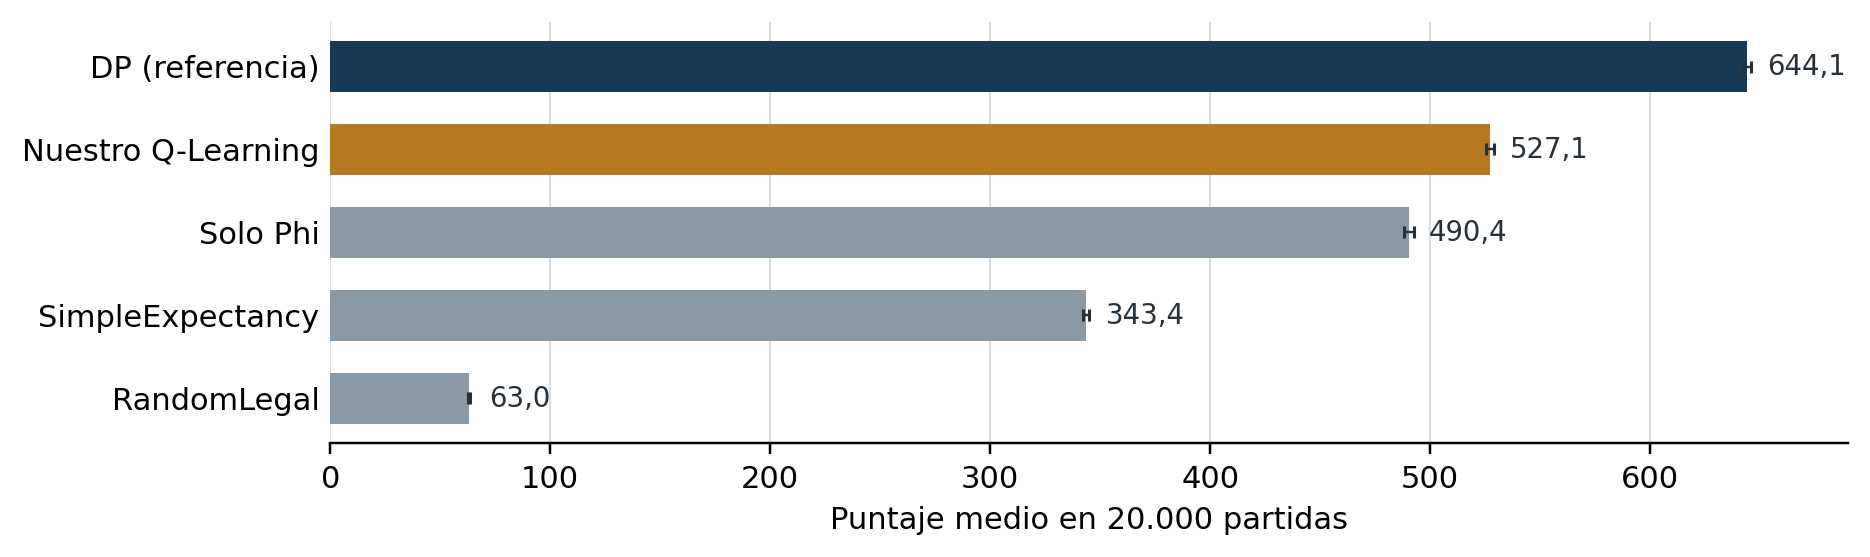
\includegraphics[width=0.88\textwidth]{grafico_resultados.png}
    \caption{Puntaje medio. La DP aparece como referencia y no como competidor.}
    \label{fig:resultados}
\end{figure}

Nuestro agente obtuvo \textbf{527,06} puntos, frente a 343,40 de \texttt{SimpleExpectancy} y 63,03 de \texttt{RandomLegal}. Representa el 82\% del valor calculado por la DP. En tres rangos de semillas consiguió 527,06, 526,27 y 525,42; esas diferencias entran en el error estadístico.

La representación aportó más que repetir episodios. Usar $\Phi$ sin valores aprendidos produce 490,41 puntos, mientras que el entrenamiento suma cerca de 37. Una tabla Q convencional con \emph{buckets} y topes chicos obtuvo entre 293 y 365. Esos límites agrupaban estados distintos del final de la partida y no podían expresar una política adecuada.

\newpage
\section{Qué nos permitió saber la DP}

La DP respondió preguntas que el puntaje por sí solo no contesta. Sabemos que 527,06 supera los baselines y también sabemos que quedan unos 116 puntos hasta la referencia. Pudimos calcular el costo de cada decisión comparando el valor de la acción elegida con el valor de la mejor acción según la DP. Llamamos \textbf{puntos perdidos por una decisión} a esa diferencia; vale cero cuando ambas elecciones coinciden.

La pérdida principal aparece cerca del turno 23. La política de la DP compra un escudo, conserva el oro y cobra en el turno 30. Nuestro agente compra pocos escudos y cobra antes. Probamos trazas de elegibilidad, más exploración y hasta cinco millones de episodios. Ninguna variante cerró la brecha. La secuencia útil exige dos decisiones coordinadas: comprar el escudo y luego ahorrar. La exploración $\varepsilon$-greedy cambia una acción por vez y visita poco esa continuación completa.

\subsection{Cómo evaluaríamos sin una DP}

Este juego ofrece una situación poco común en Reinforcement Learning: conocemos el modelo y el estado es lo bastante chico para enumerarlo. En un problema con imágenes, estados continuos, dinámica desconocida o muchos agentes, la tabla crecería de forma exponencial y tampoco conoceríamos $P(s'\mid s,a)$. Allí no podríamos calcular $U^*$.

Sin la DP habríamos conservado tres conclusiones sólidas:

\begin{itemize}[leftmargin=17pt,itemsep=1pt,topsep=1pt]
    \item nuestro agente supera los dos baselines bajo el protocolo de la cátedra;
    \item mantiene su media en semillas de desarrollo, control y prueba pública;
    \item las ablaciones muestran qué representación y qué hiperparámetros rinden mejor.
\end{itemize}

También habríamos perdido información. No podríamos afirmar que el agente alcanza el 82\% del potencial, medir los 116 puntos restantes ni localizar el error del escudo mediante valores óptimos. Trataríamos al mejor resultado observado como una referencia empírica, no como un máximo. Reportaríamos intervalos de confianza, curvas de aprendizaje y comparaciones con el mismo presupuesto de episodios. Las conclusiones serían relativas: ``mejor que estos baselines y estas variantes'', sin afirmar cercanía al óptimo.

Esta diferencia separa el rol de la DP del rol del agente. La DP aprovechó que la cátedra nos entregó un modelo pequeño y conocido. Q-Learning resolvió la tarea pedida: aprender una política a partir de interacciones y jugar luego sin consultar esa DP.

\section{Archivos entregados}

La cátedra proporcionó \texttt{config.py}, \texttt{env.py}, \texttt{agents.py}, \texttt{renderer.py}, \texttt{evaluate\_agents.py} y \texttt{run\_example.py}. Mantuvimos la lógica de \texttt{config.py} y \texttt{env.py}; agregamos \texttt{GoldDiceAgent} dentro de \texttt{agents.py}.

Sólo sumamos tres archivos Python propios:

\begin{center}
\small
\begin{tabularx}{\textwidth}{@{}lX@{}}
\toprule
Archivo & Responsabilidad \\
\midrule
\texttt{afterstate.py} & acciones legales, transición determinista, grilla de oro y $\Phi$ \\
\texttt{value\_table.py} & consulta, interpolación, actualización y persistencia de la tabla \\
\texttt{train\_qlearning.py} & entrenamiento Double Q-Learning y selección del checkpoint \\
\bottomrule
\end{tabularx}
\end{center}

\texttt{sol\_dp.cpp} contiene la referencia de programación dinámica y el archivo \texttt{gold\_dice\_agent.pkl} contiene los pesos entrenados. Los Markdown \texttt{01\_REGLAS\_OCULTAS.md}, \texttt{02\_RESULTADOS.md} y \texttt{03\_QUE\_CONSTRUIMOS.md} guardan los casos borde, las tablas completas y el inventario de funciones que no entran en estas tres carillas.

\end{document}
